\section{Solution}

```
Solution: describes your solution of the task.
Contains a detailed description of all the subtasks which have been solved and how they contribute to the solution for the given task.
The use of diagrams, figures, tables and similar is welcome as a support to your description.
```

\subsection{Development Process \& Tools}

\begin{figure}[ht!]
    \begin{description}
        \item{\textbf{ISE Project Navigator 12.4 M.81d}} \\
            Main IDE for writing and synthesizing VHDL.
        \item{\textbf{ISim 12.4 M.81d}} \\
            Simulation environment for simulating VHDL.
        \item{\textbf{hostcomm 1.0.0}} \\
            Programming utility for the Spartan-6 LX16 Evaluation Kit.
        \item{\textbf{Vim}} \\
            For text editing.
        \item{\textbf{ghdl}} \\
            Allowed for writing and testing components on Mac OS X.
        \item{\textbf{gtkwave 3.3.58}} \\
            Visualization tool for inspecting test simulations run with ghdl.
        \item{\textbf{git \& GitHub}} \\
            Version control system with central code repository hosting.
    \end{description}
    \caption{yo}
\end{figure}

\subsection{Architecture}

Utgangspunkt, endringer, hvorfor, endelig resultat

\subsubsection{MIPS subset}

\subsubsection{State machine}

A state diagram for the control unit can be seen in figure \ref{fig:state_machine}.

\begin{figure}[ht!]
    \begin{center}
    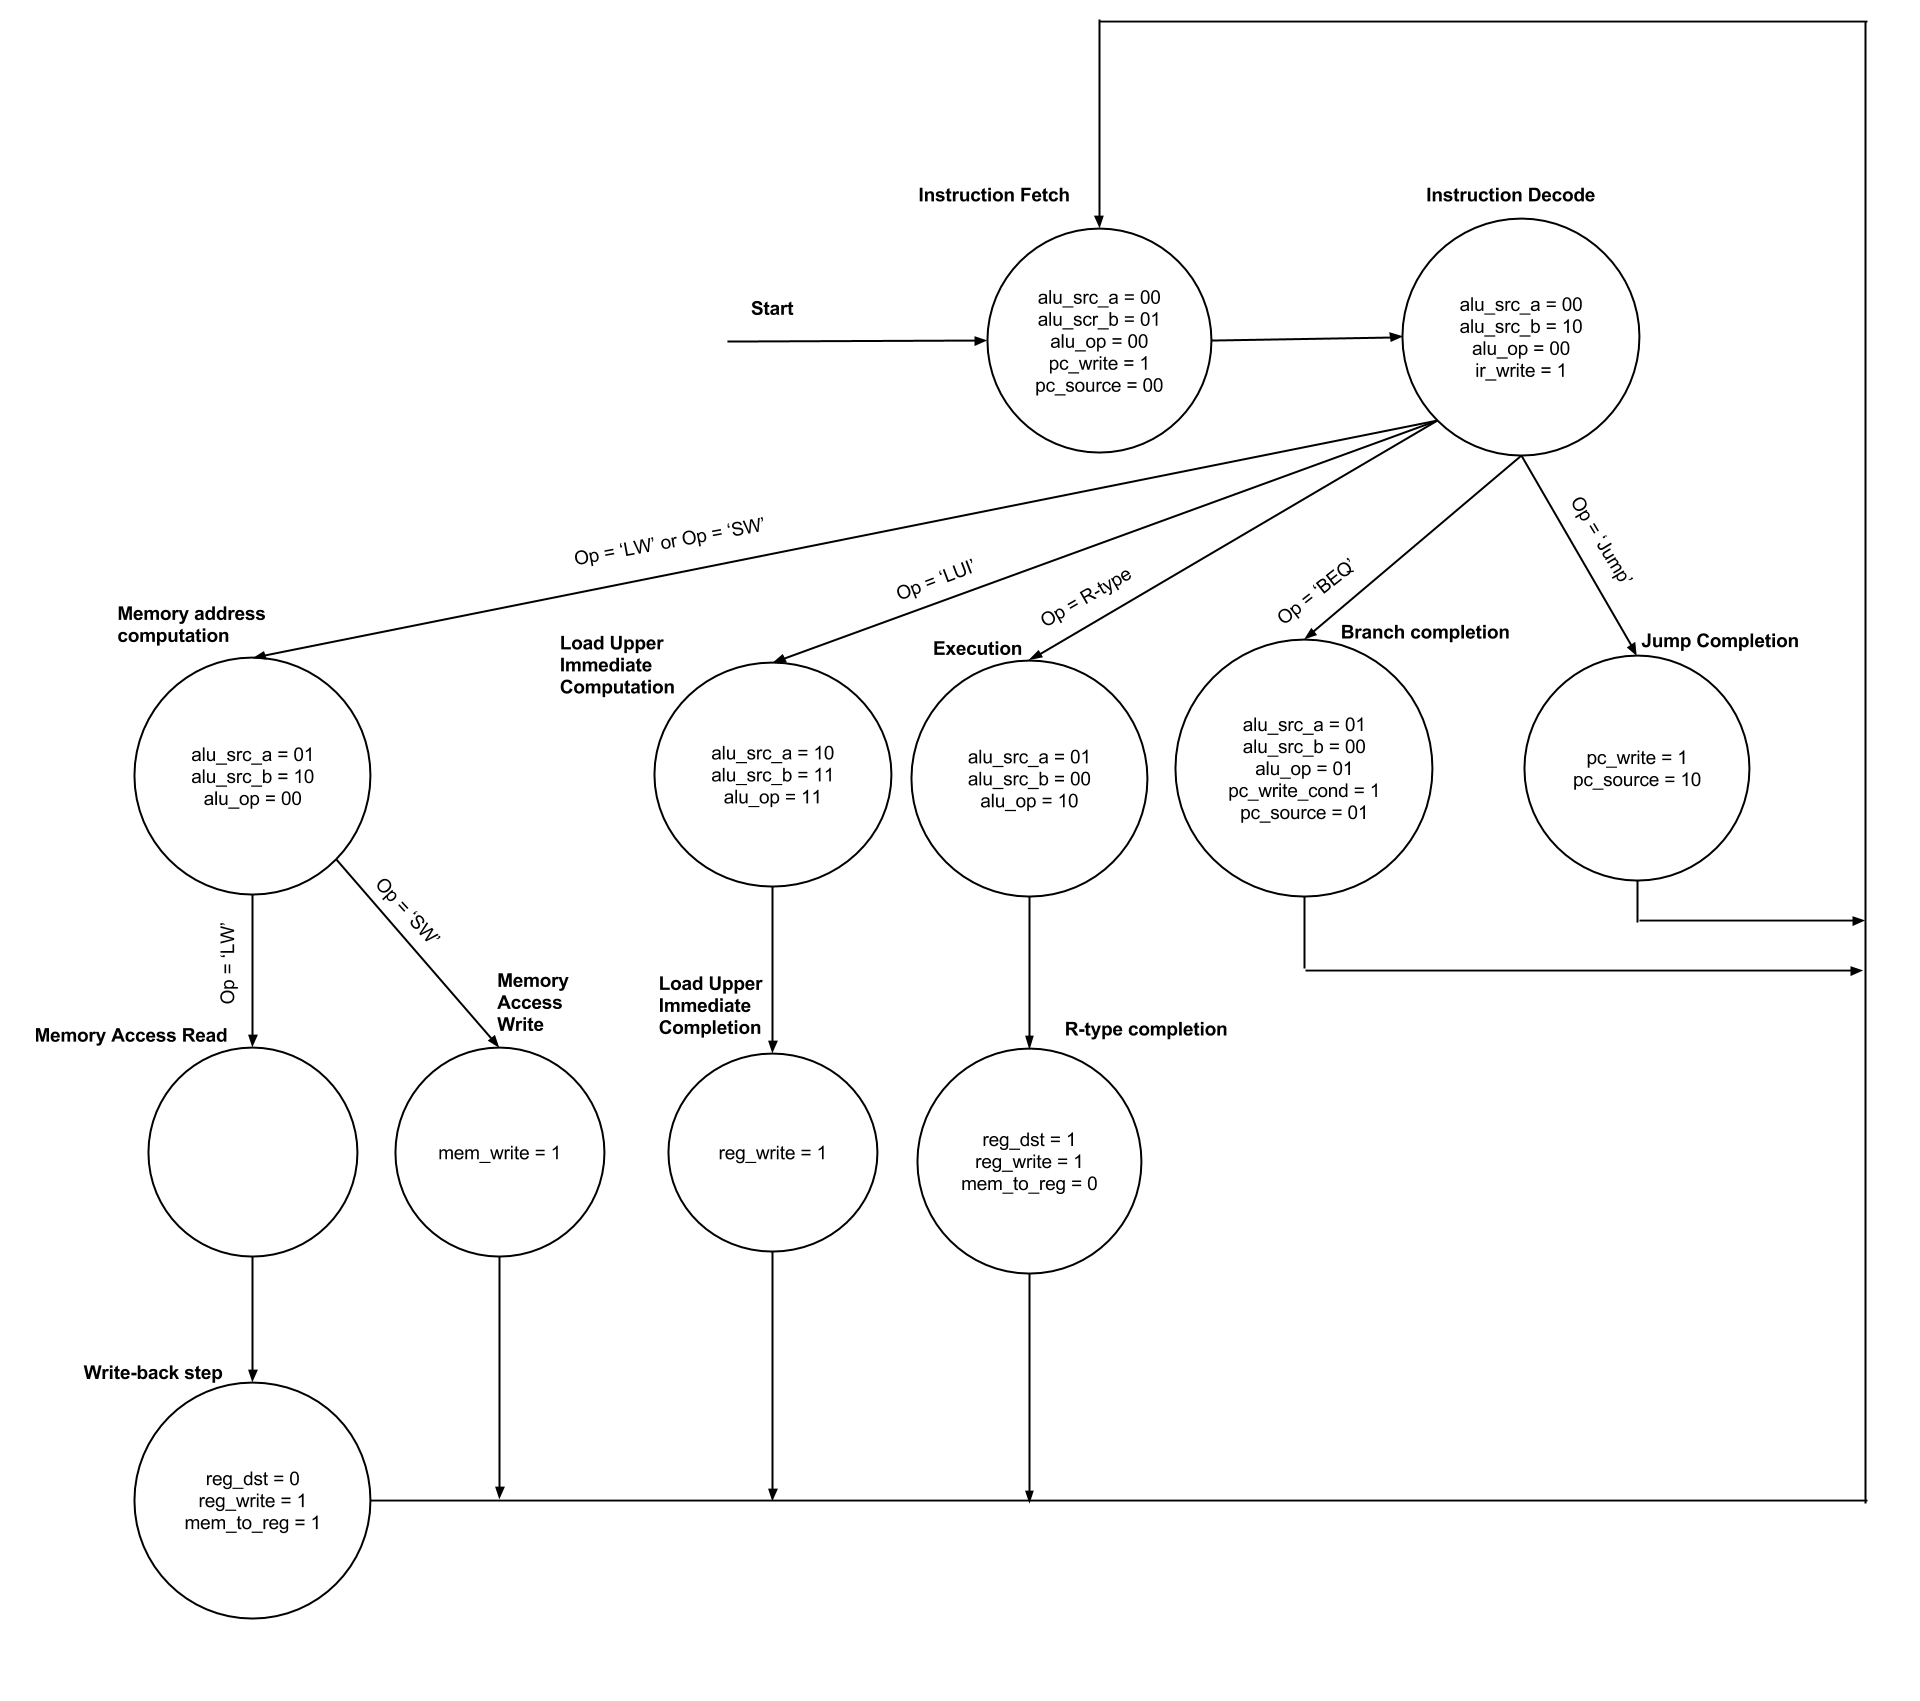
\includegraphics[width=\textwidth]{assets/state_machine.png}
    \caption{State diagram for the control unit}
    \label{fig:state_machine}
    \end{center}
\end{figure}

\subsubsection{RTL schematic}

\subsection{Implementation}

\subsubsection{Modularization}

Bottom-up approach, unit tests, integration tests

\subsection{Optimizing for FPGA}


Things to write about

\begin{enumerate}
  \item
    Chip select on ram, power savings

  \item
    The war on Xilinx ISE. Learning experiences etschetera

  \item
    Block ram in Registers instead of flip-flops with gigantic muxes. The reason for this is that a hardware designer has to consider his platform, in this case the target was an FPGA, and not 'actual' hardware. FPGAs hate muxes , altho they might be better in real hardware. like -- insert explicitive here --. Mention the LUT savings here. Like 2445 to 750 luts!!!! wow such save.

  \item
    State machine is based on the multicycle mips architecture provided in lecture slides.

  \item
    Outsourcing ALU control values to vhdl ENUM as it is better than us to assign logic values!

  \item
    Reducing critical path to increase clock frequency. Worst path is instruction immediate -> alu latch B -> alu -> zero out -> PC write.


\end{enumerate}
